\documentclass{article}

\usepackage[preprint]{neurips_2025}
\usepackage[utf8]{inputenc}
\usepackage[T1]{fontenc}
\usepackage{hyperref}
\usepackage{url}
\usepackage{booktabs}
\usepackage{amsmath}
\usepackage{amssymb}
\usepackage{graphicx}
\usepackage{microtype}
\usepackage{xcolor}

\title{Directional Writing in Gradient-Based Memory:\\A Preliminary Study on Mixed-Orientation KV Retrieval}

\author{Anonymous Author(s)}

\newcommand{\dataset}{\textsc{mix-N8}}
\newcommand{\inverse}{\textsc{inverse-N4}}
\newcommand{\egm}{EnergyGradMem}
\newcommand{\gm}{GradMem}

\begin{document}
\maketitle

\begin{abstract}
Gradient-based memory compresses a context by optimizing a small, per-example memory state under a self-supervised WRITE loss.  Standard autoregressive reconstruction makes this operation direction-sensitive: it naturally predicts the right side of a key--value pair from the left side.  We introduce \dataset, where each context is either forward, \texttt{F!KK:VV!}, or backward, \texttt{B!VV:KK!}, while every query asks for \texttt{VV} given \texttt{KK}.  The task therefore requires one model to handle both context orientations.  Both available ordinary reconstruction \gm{} seeds plateau near 56\% exact match (EM), whereas one of three same-configuration \egm{} seeds reaches 96.4\% EM and the other two remain near 13\%.  A frozen-checkpoint decomposition shows that \gm{} is perfect on forward examples but only 15.3\% EM on backward examples; its WRITE steps reduce value-token reconstruction loss while leaving key-token loss almost unchanged.  The successful energy checkpoint instead solves both orientations, but exhibits initial memory-gradient norms above $10^3$; semantic key and value energies rise after step one and partially return after step two.  Lipschitz regularization and memory-update noise have not produced independent convergence from scratch.  These results provide a proof of possibility for the evaluated learned, label-free WRITE configuration, not evidence that energy is generally superior: the central limitation is severe optimization instability and seed sensitivity.
\end{abstract}

\section{Introduction}
\label{sec:introduction}

\gm{} learns to compress a context $C$ into a compact memory $M$ by differentiating through test-time gradient descent \cite{kuratov2026gradmem}.  Starting from a shared initialization $M_0$, WRITE performs $K$ updates while model parameters are fixed; READ then predicts a target from the optimized memory and query, without access to the original context.  The standard inner objective is autoregressive reconstruction,
\begin{equation}
  \mathcal{L}_{\mathrm{rec}}(M;C)
  = -\sum_i \log p(c_i\mid M,c_{<i}),
  \qquad
  M_{k+1}=M_k-\eta\nabla_M\mathcal{L}_{\mathrm{rec}}(M_k;C).
\end{equation}
This objective is not direction-neutral.  In a pair \texttt{KK:VV}, predicting later tokens allows the WRITE gradient to encode information useful for recovering \texttt{VV} from \texttt{KK}.  Reversing the pair to \texttt{VV:KK} breaks this alignment: reconstruction can predict the key from the preceding value, while downstream READ requires the opposite association.

Prior \inverse{} experiments show that this mismatch is not an absolute impossibility.  With only \texttt{VV:KK} pairs, two of three comparable reconstruction \gm{} runs reach approximately 99\% EM, and write-head variants reach 100\% EM.  The model can therefore meta-learn a right-to-left-effective update when orientation is globally consistent.  The open question is whether one WRITE rule can support both directions on a per-example basis.

We study this question on \dataset{} and audit the current stabilization attempts.  Our main observations are:
\begin{enumerate}
  \item Both available reconstruction \gm{} seeds reach a similar aggregate plateau; a frozen subset evaluation obtains 100\% EM on forward examples and 15.3\% on backward examples.
  \item A single \egm{} seed reaches 96.4\% validation EM, demonstrating that the evaluated configuration can compress both orientations, but two same-configuration seeds fail near 13\% EM.
  \item The successful energy dynamics have initial gradient norms above $10^3$ in both orientations.  Semantic key and value energies rise after the first step and partially return after the second.
  \item Current Lipschitz and noise interventions do not establish improved convergence from scratch.  The best 98.1\% EM memory-search result starts from the successful plateau and uses target-guided outer-loop teachers unavailable at inference; its forward WRITE trajectory remains context-only because teacher-for-next-step is disabled.
\end{enumerate}

\section{Mixed-Orientation KV Retrieval}
\label{sec:task}

Each \dataset{} context contains eight two-character key--value pairs and an orientation prefix.  Forward examples have the form
\begin{center}
\texttt{F!KK:VV!!KK:VV!...},
\end{center}
and backward examples have the form
\begin{center}
\texttt{B!VV:KK!!VV:KK!...}.
\end{center}
The query is always \texttt{?!KK:} and the target is \texttt{VV!|}.  Keys are unique within an example; the character vocabulary has 62 symbols.  There are $10^6$ training examples and 5,000 validation examples.  The direction marker makes the required transformation observable from $C$, while WRITE remains query-independent.

The task distinguishes three possibilities.  First, a model may learn only the autoregressively convenient forward write.  Second, it may settle on a direction-agnostic compromise.  Third, it may use the prefix to select an orientation-conditioned update field.  Because READ never receives $C$, success requires WRITE to place the correct association in memory rather than deferring orientation handling to READ.

\section{Methods}
\label{sec:methods}

\paragraph{Reconstruction \gm.}
The baseline minimizes context reconstruction cross-entropy during WRITE.  Unless noted otherwise, the principal comparison uses a four-layer Llama-style transformer with four attention heads, hidden dimension 256, eight input-prefix memory tokens, $K=2$ SGD WRITE steps, inner learning rate $\eta=0.4$, full second-order differentiation, batch size 64, and outer learning rate $10^{-4}$ in fp32.  The reconstruction runs load a pretrained Llama checkpoint, while the principal energy runs start without that initialization; the successful energy configuration also uses auxiliary losses described below.  The comparison therefore does not isolate WRITE objective choice.

\paragraph{EnergyGradMem.}
\egm{} replaces reconstruction with a learned scalar energy.  A learned head scores each context hidden state, applies a softplus, and averages over non-padding context tokens:
\begin{equation}
  E_\theta(M;C)=\frac{1}{|C|}\sum_i
  \operatorname{softplus}\!\left(h_\theta(z_i(M,C))\right),
  \qquad M_{k+1}=M_k-\eta\nabla_M E_\theta(M_k;C).
\end{equation}
WRITE uses context but no query or target.  READ target cross-entropy meta-trains the transformer, memory initialization, and energy head through the WRITE trajectory.  The successful configuration also uses step-alignment and intermediate-READ auxiliary weights of 0.1 each.  These are outer training signals; inference-time WRITE remains context-only.

\paragraph{Stabilization attempts.}
The Lipschitz penalty directly constrains $\lVert\nabla_M E\rVert_2$ at the detached final WRITE state $M_K$, with weight 0.003 and threshold 5.  Memory noise injects Gaussian perturbations into updates with scale 0.03.  Memory search samples four norm-scaled perturbations around each post-update state and matches WRITE to a lower-READ-loss detached teacher.  All reported search runs use radius scale 0.25 and minimum relative target gain 0.3.  Plateau-initialized search uses weight 1.0 with gain weighting; the scratch noise-plus-search run uses weight 0.1 without gain weighting.

\paragraph{Metrics and checkpoint analysis.}
We report token accuracy and exact match on the two target characters, excluding formatting tokens.  Tables use the best recorded validation checkpoint unless stated otherwise.  For mechanistic analysis, we replay frozen WRITE trajectories on the first 256 validation examples (132 forward and 124 backward), preserving production token alignment and softplus energy.  We parse semantic key and value spans rather than fixed positions, and report token-level reconstruction CE, energy, and memory-gradient norm at $M_0,M_1,M_2$, plus final-READ accuracy by orientation.  This subset was selected deterministically rather than sampled; it is diagnostic and should not replace full-validation metrics.

\section{Results}
\label{sec:results}

\subsection{Inverse-only retrieval is learnable}

Table~\ref{tab:inverse} confirms the premise of the mixed task.  On \inverse{}, where every pair is written \texttt{VV:KK}, reconstruction \gm{} succeeds in two of three matched runs; a separate write-head configuration succeeds in both available runs.  Thus ordinary \gm{} can meta-learn updates useful for inverse retrieval when the entire task distribution has one orientation.  The failed seeds nevertheless show that even the simpler inverse task is not uniformly stable.

\begin{table}[t]
  \caption{Best validation exact match on \inverse{}.  Seeds correspond to run indices 1--3 (143--145).  Mean and sample standard deviation are descriptive over the available runs, not uncertainty estimates.}
  \label{tab:inverse}
  \centering
  \small
  \begin{tabular}{lrrrr}
    \toprule
    Method & Seed 143 & Seed 144 & Seed 145 & Mean $\pm$ SD \\
    \midrule
    \gm{} reconstruction + auxiliaries & 99.02 & 26.56 & 99.22 & $74.93\pm41.89$ \\
    \gm{} reconstruction, write head & 100.00 & 100.00 & --- & $100.00\pm0.00$ \\
    \egm{} & 97.20 & 99.00 & 41.54 & $79.25\pm32.67$ \\
    \bottomrule
  \end{tabular}
\end{table}

\subsection{Mix-N8 has a baseline plateau and a rare energy solution}

Table~\ref{tab:mix-main} summarizes the principal 256-dimensional experiments.  Both available reconstruction \gm{} seeds plateau at about 56\% EM.  \egm{} has a much higher maximum but a lower mean and enormous variance: only seed 144 enters the high-accuracy regime.  Consequently, the current evidence supports a proof of possibility, not a method-level advantage.  The successful run peaks at 96.40\% EM and 98.17\% token accuracy at step 833,500, then finishes its recorded trajectory at 95.78\% EM.  It does not reach the 99\% stopping threshold.  Architecture and core optimization settings are shared, but initialization and auxiliary outer losses differ between method families.

Figure~\ref{fig:learning-curves} shows that the difference is not a small shift in asymptotic accuracy.  Both reconstruction runs rapidly enter the same plateau, while two energy seeds remain in a low-accuracy regime.  Energy seed 144 passes through an extended intermediate regime and then undergoes a sharp transition after roughly 180,000 outer steps, eventually approaching but not reaching the 99\% stopping target.  This history motivates treating convergence probability and time-to-transition as primary metrics.

\begin{figure}[t]
  \centering
  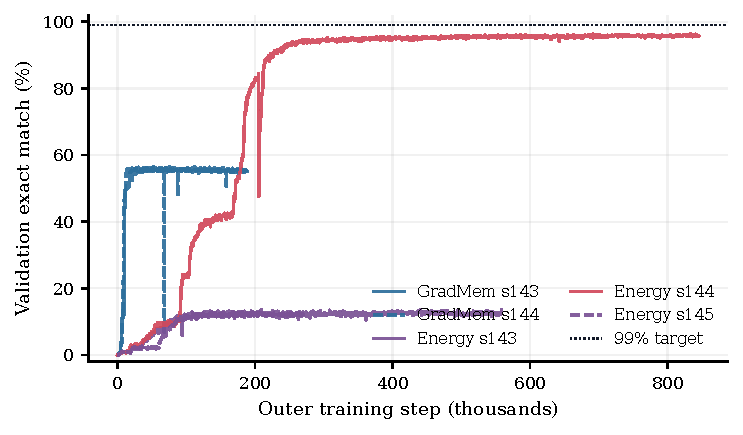
\includegraphics[width=0.88\linewidth]{figures/learning_curves.pdf}
  \caption{Full-validation exact-match histories for the principal \dataset{} runs.  Curves are unsmoothed evaluations recorded every 500 outer steps.  Both available reconstruction seeds plateau near 56\% EM; only energy seed 144 enters the high-accuracy regime.  Method families differ in initialization and auxiliary losses as described in Section~\ref{sec:methods}.}
  \label{fig:learning-curves}
\end{figure}

\begin{table}[t]
  \caption{Best validation performance on \dataset{} for the principal configurations.  Values are percentages.  Energy seeds are mutually matched; cross-method initialization and auxiliary losses differ.}
  \label{tab:mix-main}
  \centering
  \small
  \begin{tabular}{lrrrrr}
    \toprule
    Method & Seed 143 EM & Seed 144 EM & Seed 145 EM & Mean $\pm$ SD & Best token acc. \\
    \midrule
    \gm{} reconstruction & 56.12 & 56.20 & --- & $56.16\pm0.06$ & 77.87 \\
    \gm{} reconstruction, write head & 56.36 & 56.50 & --- & $56.43\pm0.10$ & 77.85 \\
    \egm{} & 13.44 & \textbf{96.40} & 13.60 & $41.15\pm47.85$ & \textbf{98.17} \\
    \bottomrule
  \end{tabular}
\end{table}

The approximately 56\% aggregate baseline masks a clean directional split.  On the frozen 256-example subset, reconstruction \gm{} obtains 100\% EM on forward contexts but 15.32\% on backward contexts (Table~\ref{tab:direction}).  The successful energy checkpoint obtains 90.91\% and 100\%, respectively.  The failed energy seed remains poor in both directions.  This rules out the simplest account that the successful run merely switched from forward to backward preference: it learned to handle both orientations.

\begin{table}[t]
  \caption{Orientation-conditioned frozen-checkpoint metrics on the first 256 \dataset{} validation examples.  The subset contains 132 forward and 124 backward examples.}
  \label{tab:direction}
  \centering
  \small
  \begin{tabular}{lrrrr}
    \toprule
    Checkpoint & F token acc. & F EM & B token acc. & B EM \\
    \midrule
    \gm{} best (seed 143) & 100.00 & 100.00 & 57.66 & 15.32 \\
    \egm{} failed (seed 143) & 53.41 & 10.61 & 56.85 & 16.13 \\
    \egm{} successful (seed 144) & 95.45 & 90.91 & 100.00 & 100.00 \\
    \bottomrule
  \end{tabular}
\end{table}

\paragraph{Evaluation-time WRITE steps.}
Figure~\ref{fig:k-sweep} evaluates the same frozen checkpoints with $K\in\{0,1,2,4,8\}$, although all were trained with $K=2$.  Without WRITE ($K=0$), every checkpoint has zero EM.  Reconstruction \gm{} reaches 100\% forward EM by $K=2$ but remains at 15.3\% backward EM through $K=4$.  The successful energy checkpoint reaches 88.6\% forward and 99.2\% backward EM at $K=1$, 90.9\% and 100\% at $K=2$, and 78.8\% and 99.2\% at $K=8$.  The small $K=1$ versus $K=2$ difference corresponds to only three forward examples and should not be overinterpreted; the larger $K=8$ decline is evidence of sensitivity beyond the trained unroll horizon, not a comparison against a model trained or step-size-tuned for $K=8$.

\begin{figure}[t]
  \centering
  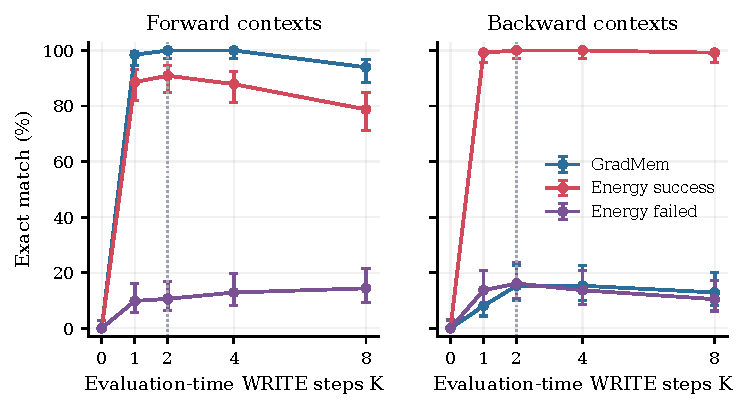
\includegraphics[width=0.92\linewidth]{figures/exact_match_vs_k.pdf}
  \caption{Orientation-conditioned exact match versus evaluation-time WRITE steps on the fixed 256-example diagnostic subset.  Error bars are 95\% Wilson binomial intervals; evaluations at different $K$ use the same examples and are therefore paired.  The vertical dotted line marks training $K=2$.  Values for $K>2$ probe off-training-horizon dynamics at unmatched WRITE compute and without retuning the inner learning rate.}
  \label{fig:k-sweep}
\end{figure}

\subsection{WRITE decompositions expose different failure modes}

Table~\ref{tab:components} separates semantic key and value tokens along the frozen trajectory.  Direction-aware masks were audited over all 5,000 validation examples: \texttt{F} assigns the left field to keys and the right field to values, while \texttt{B} swaps those semantic roles.  Reconstruction \gm{} leaves key CE almost unchanged and key top-1 WRITE accuracy at 0\%, but sharply improves value reconstruction in both syntactic orientations.  For forward examples, this is aligned with retrieval because value tokens follow key tokens.  In backward examples, WRITE directly optimizes reconstruction of the left-side value tokens and raises their accuracy to 56.8\%, but this does not imply that memory supports the required key-to-value lookup: final READ backward EM remains 15.3\%.  READ predicts values from queried keys and never attempts to reconstruct context keys.

\begin{table}[t]
  \caption{Frozen WRITE diagnostics at $M_0\rightarrow M_1\rightarrow M_2$ on 256 examples.  CE is token reconstruction loss; parenthesized values show top-1 WRITE reconstruction accuracy for \gm{}; $E_K,E_V$ are token energies; $\lVert g\rVert$ is the mean per-example memory-gradient norm.}
  \label{tab:components}
  \centering
  \small
  \begin{tabular}{llrrrrr}
    \toprule
    Checkpoint & Dir. & Key CE (\gm{} acc.) & Value CE (\gm{} acc.) & $E_K$ & $E_V$ & $\lVert g\rVert$ \\
    \midrule
    \gm{} & F & $4.34\!\to\!4.35\!\to\!4.34$ (0.0\%) & $4.47\!\to\!1.11\!\to\!0.64$ (0.0$\to$98.4\%) & --- & --- & $2.62\!\to\!0.78\!\to\!0.43$ \\
    \gm{} & B & $4.65\!\to\!4.63\!\to\!4.62$ (0.0\%) & $4.23\!\to\!1.61\!\to\!1.43$ (1.1$\to$56.8\%) & --- & --- & $2.19\!\to\!0.45\!\to\!0.31$ \\
    \egm{} success & F & $15.65\!\to\!14.13\!\to\!13.52$ & $7.62\!\to\!6.15\!\to\!5.16$ & $2035\!\to\!7765\!\to\!4682$ & $3645\!\to\!8941\!\to\!6240$ & $1121\!\to\!93.5\!\to\!42.8$ \\
    \egm{} success & B & $8.33\!\to\!8.42\!\to\!7.57$ & $14.72\!\to\!11.47\!\to\!10.79$ & $3309\!\to\!4666\!\to\!2674$ & $3377\!\to\!5504\!\to\!3254$ & $1286\!\to\!76.8\!\to\!40.4$ \\
    \bottomrule
  \end{tabular}
\end{table}

The energy solution is qualitatively different.  At $M_0$, mean gradient norms are 1,121 for forward and 1,286 for backward examples, approximately 400--600 times larger than reconstruction \gm{}.  With $\eta=0.4$, the first update moves far enough that both semantic key and value energies increase substantially.  The second update partially returns, but these component energies do not uniformly fall below $M_0$.  This behavior is consistent with discrete-time overshoot and with the checkpoint's logged positive final-minus-initial full energy, although the component probe does not record the complete scalar objective at every step.  It also implies that a pointwise post-WRITE Lipschitz penalty is aimed at only part of the problem: the dangerous region is already encountered at $M_0$ and along the first segment.

Figure~\ref{fig:write-diagnostics} visualizes these two mechanisms directly.  Reconstruction's forward value CE collapses while key CE remains flat.  In the successful energy checkpoint, both semantic energy components increase sharply at $M_1$ before partially returning.  The log-scale gradient panel emphasizes that both successful and failed energy checkpoints operate at a qualitatively different scale from reconstruction \gm{}.

\begin{figure}[t]
  \centering
  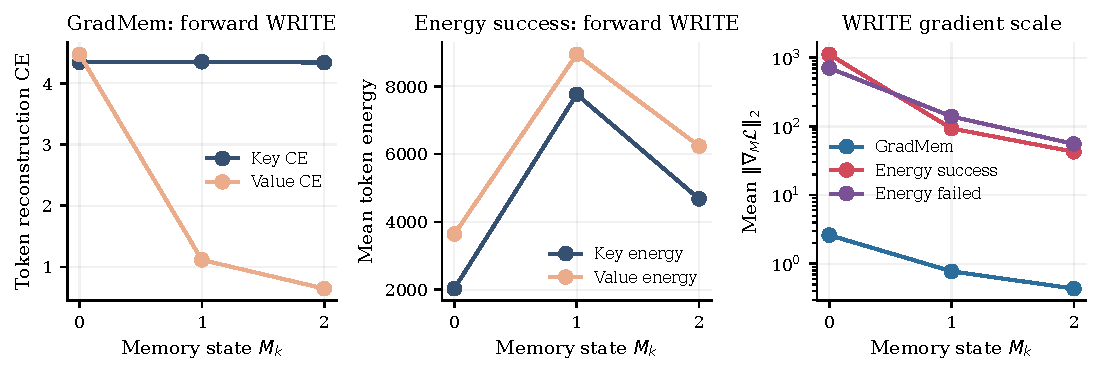
\includegraphics[width=\linewidth]{figures/write_diagnostics.pdf}
  \caption{Frozen forward-context WRITE diagnostics on 132 examples from the 256-example subset.  Left: reconstruction \gm{} reduces value CE but not key CE.  Center: semantic key and value energies in the successful energy checkpoint overshoot after the first update.  Right: mean memory-gradient norms are shown on a logarithmic scale.  Energy values are checkpoint-specific and should be interpreted with the fixed inner learning rate $\eta=0.4$.}
  \label{fig:write-diagnostics}
\end{figure}

The failed energy checkpoint displays another degeneracy.  Its forward key energy at $M_0$ is approximately $1.3\times10^{-21}$ while forward value energy is 3,657, an extreme token-role imbalance.  The successful model has large energies on both roles and an orientation-dependent profile.  Absolute energy scale is not identifiable from READ utility alone, and softplus permits saturation near zero, so unconstrained energy learning can create flat token regions alongside very steep memory gradients elsewhere.

\subsection{Current stabilization evidence}

Table~\ref{tab:stability} separates interventions trained from scratch from those initialized at the successful seed-144 plateau.  Lipschitz regularization from scratch remains in the low regime (10.7--12.4\% EM).  Adding memory noise lowers the observed best to 8.8\% EM in the one completed run.  High EM after plateau initialization mostly demonstrates retention of an existing solution: Lipschitz and Lipschitz-plus-noise peak at 96.1\% and 95.7\%, respectively, without exceeding the original 96.4\% EM.

\begin{table}[t]
  \caption{Best \dataset{} validation EM for stabilization experiments.  ``Plateau init.'' loads the already successful seed-144 checkpoint at step 534,500.}
  \label{tab:stability}
  \centering
  \small
  \begin{tabular}{llrr}
    \toprule
    Intervention & Initialization & Runs & Best EM range \\
    \midrule
    Lipschitz ($\lambda=0.003,L=5$) & scratch & 2 & 10.72--12.38 \\
    Lipschitz + noise ($\sigma=0.03$) & scratch & 1 & 8.82 \\
    Lipschitz + noise + search & scratch & 1 & 11.64 \\
    Lipschitz & plateau & 2 & 95.70--96.08 \\
    Lipschitz + noise & plateau & 1 & 95.66 \\
    Lipschitz + memory search & plateau & 2 & 94.92--98.10 \\
    \bottomrule
  \end{tabular}
\end{table}

Figure~\ref{fig:stability} makes the initialization confound explicit.  Every completed scratch intervention remains below 13\% EM, whereas every plateau-initialized intervention remains above 94\%.  Individual points are available runs and vertical segments show observed ranges where two runs exist.  The visual separation should not be read as a treatment effect because the two panels begin from qualitatively different checkpoints.

\begin{figure}[t]
  \centering
  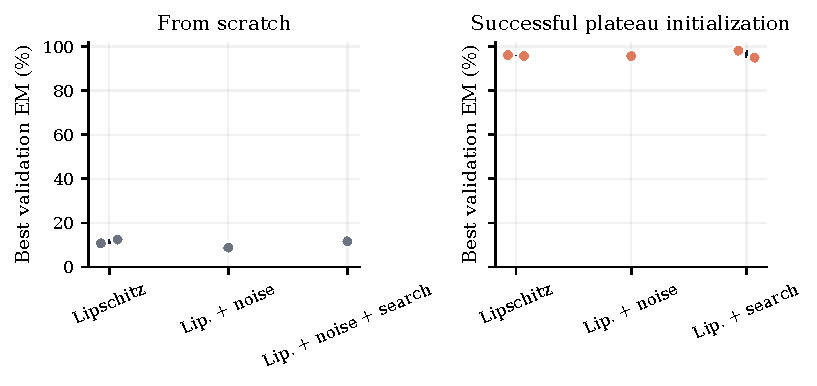
\includegraphics[width=0.88\linewidth]{figures/stability_interventions.pdf}
  \caption{Best validation EM for completed stabilization runs, separated by initialization.  Points are individual runs and vertical segments are observed ranges.  Both panels share a 0--100\% scale.  From-scratch interventions do not enter the high-accuracy regime; plateau-initialized runs primarily retain an existing solution.}
  \label{fig:stability}
\end{figure}

The best observed result, 98.10\% EM, uses memory search after plateau initialization.  It should be interpreted carefully.  Search selects perturbations using READ targets to construct a detached outer-loop teacher.  In the reported configuration, it does not replace inference-time WRITE and does not use the selected teacher as the next-step forward state, but it still supplies target-guided training supervision unavailable at inference.  The result is useful evidence that better local memory states exist near the learned trajectory; it is not evidence that the context-only energy dynamics can reliably discover them from scratch.  Two combined search/noise runs failed at step zero due to GPU out-of-memory caused by an occupied device and therefore provide no algorithmic evidence.

\subsection{WRITE-step extrapolation from the successful plateau}
\label{sec:plateau-extrapolation}

We directly compare the exact initialization used by all plateau descendants, \texttt{run\_2\_unfinished/checkpoint-534500}, against five best descendant checkpoints.  Every model was trained with $K=2$ and is evaluated frozen at $K\in\{0,1,2,4,8\}$ on the same 256 examples.  This is extrapolation in unroll depth, not context length; $K>2$ uses unmatched WRITE compute and no step-size retuning.

Among these selected checkpoints, the two plain Lipschitz descendants show the most stable observed repeated-WRITE dynamics.  Both retain 100\% backward EM through $K=8$, while forward EM remains between 88.6\% and 90.9\% for $K=2,4,8$.  The initialization itself is also fairly stable, declining from 100\% to 96.0\% backward EM and from 87.9\% to 87.1\% forward EM between $K=2$ and $K=8$.  The noise descendant behaves similarly.  Memory search seed 143 has the highest observed forward EM, 97.7\% at $K=4$ (97.0\% at the trained horizon), but declines to 91.7\% forward and 91.1\% backward at $K=8$.  Its seed-144 realization is much less stable: backward EM falls from 99.2\% at $K=2$ to 20.2\% at $K=8$.  The selected memory-search checkpoints can therefore combine strong trained-horizon quality with unstable repeated application; this descriptive comparison does not isolate the intervention.

\begin{figure}[t]
  \centering
  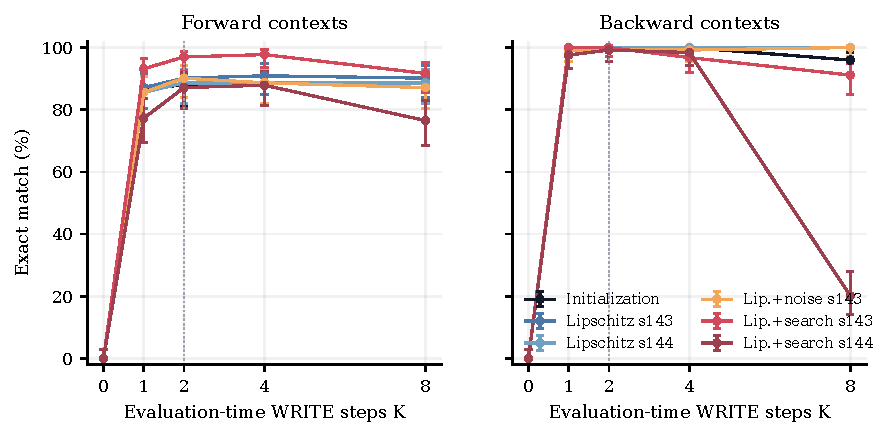
\includegraphics[width=\linewidth]{figures/plateau_write_step_extrapolation.pdf}
  \caption{Frozen WRITE-step extrapolation for the common successful initialization and all five selected direct plateau descendants.  Error bars are 95\% Wilson intervals on a fixed subset of 132 forward and 124 backward examples; they do not represent training-seed or checkpoint-selection uncertainty.  The dotted line marks training $K=2$.  Every descendant inherits the same seed-144 initialization; suffixes denote post-initialization RNG seeds, and seed-143 descendants are not seed-matched intervention controls.}
  \label{fig:plateau-extrapolation}
\end{figure}

\subsection{Local WRITE and READ loss slices}
\label{sec:landscapes}

We probe three seed-144 checkpoints: the common initialization, its plain Lipschitz descendant, and its Lipschitz-plus-search descendant.  For each of 12 fixed examples (five forward, seven backward), we replay through $M_8$ and analyze the intervals $M_0\to M_1$, $M_1\to M_2$, $M_2\to M_4$, and $M_4\to M_8$.  For each interval $(a,b)$ we independently define
\begin{equation}
 b_x^{a:b}=M_b-M_a,\qquad
 b_y\perp b_x,\qquad \lVert b_y\rVert_2=\lVert b_x\rVert_2,
\end{equation}
where each example and interval has a separately seeded random orthogonal direction $b_y$.  We evaluate
\begin{equation}
  P_{a:b}(x,y)=M_a+x b_x^{a:b}+y b_y^{a:b},\qquad (x,y)\in[-3,3]^2.
\end{equation}
Thus every row uses its corresponding trajectory interval as the horizontal axis: $(0,0)=M_a$ and $(1,0)=M_b$ exactly.  The $2\to4$ and $4\to8$ rows represent multi-update displacements, not single gradient steps.  Each contour is the mean of 12 per-example centered loss-change slices in normalized coordinates, not one shared global plane; losses are center-subtracted but not scale-normalized.

Figure~\ref{fig:lipschitz-trajectory} quantifies the visited trajectory.  On this subset, the initialization has mean gradient norms $816.7\to68.9\to30.2\to18.4\to11.6$ at $K=0,1,2,4,8$.  Its first interval is very large (326.7), but later interval displacements are 27.6, 20.7, and 23.8.  Inner energy overshoots from 1,061.6 to 2,747.9, then descends to 692.0 by $M_8$; READ loss remains near zero after $M_1$.  At the currently retained seed-144 plain-Lipschitz checkpoint (step 166,000), mean gradient norms are $780.4\to26.0\to3.66\to3.27\to3.17$.  Its interval displacements contract from 312.2 to 10.4, 2.82, and 5.10, while energy descends monotonically from 876.0 to 136.1 and READ loss continues decreasing.  These are observed pointwise means, not a global Lipschitz bound or an isolated causal effect.

The Lipschitz-plus-search descendant changes scale much more dramatically and non-uniformly.  Its mean gradient norms are $1.09\to0.20\to0.14\to0.53\to0.47$.  The first three analyzed interval displacements are only 0.434, 0.080, and 0.098, and READ loss falls from 7.44 to nearly zero by $M_2$.  However, the $M_4\to M_8$ displacement explodes to 445.1 and READ loss rises from approximately zero to 1.90.  This delayed instability mirrors the seed-144 checkpoint's $K=8$ retrieval collapse.  Its energy changes little through $M_4$ ($793.04\to792.93$) and falls to 779.45 at $M_8$ even as READ worsens, showing that continued energy minimization can become misaligned with outer utility off the trained horizon.

\begin{figure}[t]
  \centering
  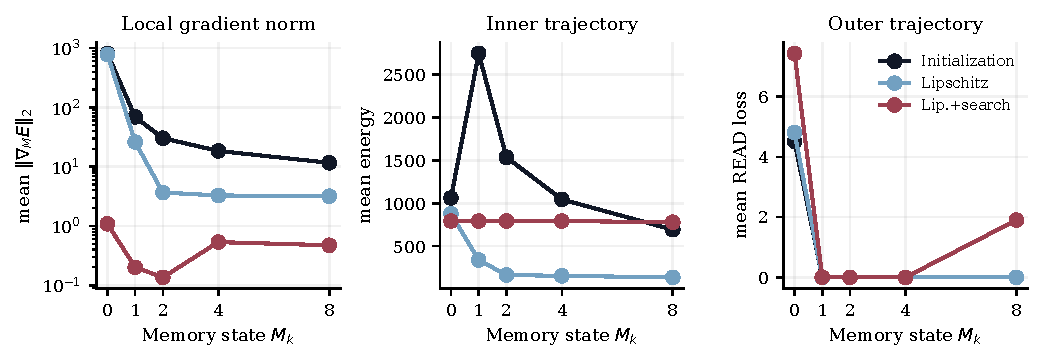
\includegraphics[width=\linewidth]{figures/lipschitz_trajectory.pdf}
  \caption{Observed trajectory statistics through evaluation-time $K=8$ on 12 examples for the seed-144 initialization and descendants.  Left: mean pointwise memory-gradient norm on a log scale.  Center: mean context-only energy.  Right: mean query-target READ loss.  All models use inner learning rate 0.4.  The search descendant's READ loss re-emerges at $M_8$ despite lower energy.}
  \label{fig:lipschitz-trajectory}
\end{figure}

Figures~\ref{fig:landscape-init}--\ref{fig:landscape-search} show the interval-specific slices.  The initialization's $0\to1$ interval overshoots to higher energy while sharply improving READ, after which its shorter intervals continue toward lower energy with little outer-loss change.  At the plain Lipschitz descendant, every displayed endpoint $(1,0)$ follows the corresponding energy-descent interval, and the small $2\to4$ and $4\to8$ scales make the later surfaces nearly flat at the shared checkpoint-level color scale.  This supports stable observed local optimization along these selected interval directions, but does not establish a per-example or continuous local minimum.

The search descendant's first three interval plots use sub-unit physical scales, but the $4\to8$ row uses mean L2 scale 445.1.  This row exposes the off-horizon failure: its endpoint lowers mean energy but raises mean READ loss.  The surfaces cannot establish global smoothness or per-example alignment: they average signed changes over different per-example planes, contain no population uncertainty, and cover one seeded orthogonal direction per example and interval.

\begin{figure}[p]
  \centering
  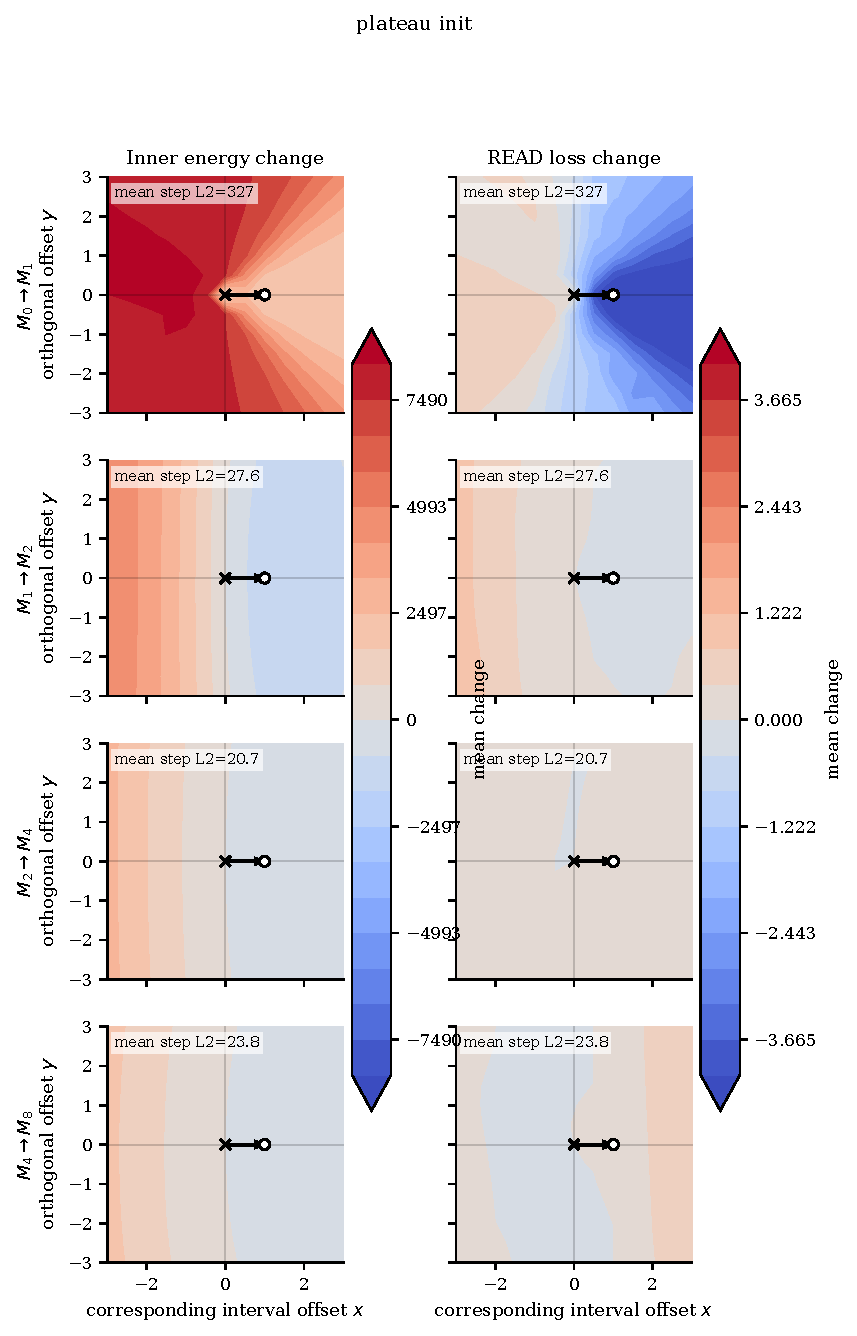
\includegraphics[width=0.82\linewidth]{figures/landscape_plateau-init.pdf}
  \caption{Mean of 12 per-example centered loss-change slices for the plateau initialization.  Rows use the corresponding $0\to1$, $1\to2$, $2\to4$, and $4\to8$ interval directions.  In every row the cross at $(0,0)$ is the start and the white point at $(1,0)$ is exactly the endpoint.  The inset reports the mean interval L2 norm; one coordinate unit uses each example's own interval norm.  Color scales are checkpoint-specific, symmetric, and saturated beyond the 97th absolute percentile.}
  \label{fig:landscape-init}
\end{figure}

\begin{figure}[p]
  \centering
  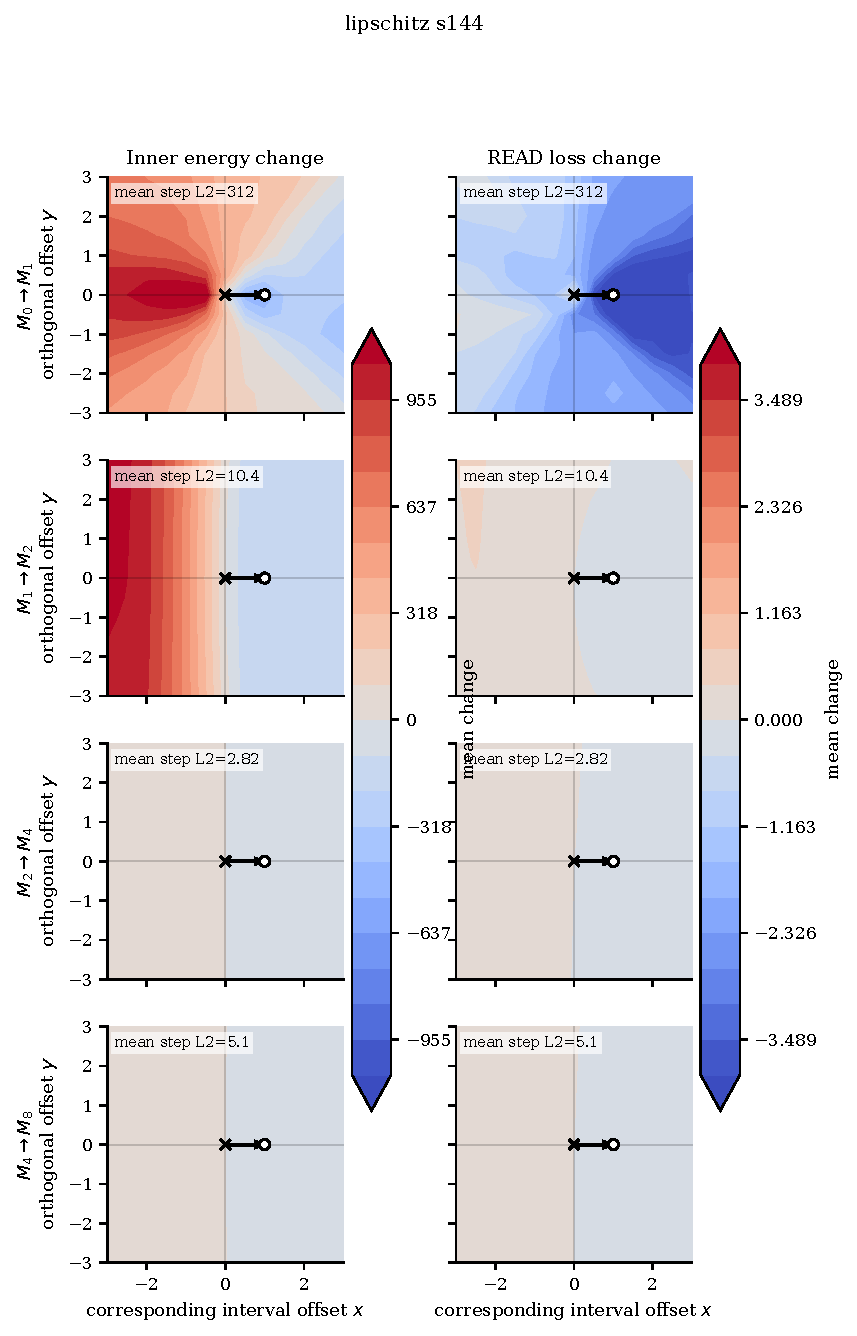
\includegraphics[width=0.82\linewidth]{figures/landscape_lipschitz-s144.pdf}
  \caption{Transition-specific slices for the currently retained seed-144 plain-Lipschitz best checkpoint (step 166,000).  Every row uses its corresponding interval as the horizontal axis and an independently seeded equal-norm orthogonal direction.  Mean interval norms are shown in-panel.  Color scales are checkpoint-specific and saturated beyond the 97th absolute percentile.}
  \label{fig:landscape-lipschitz}
\end{figure}

\begin{figure}[p]
  \centering
  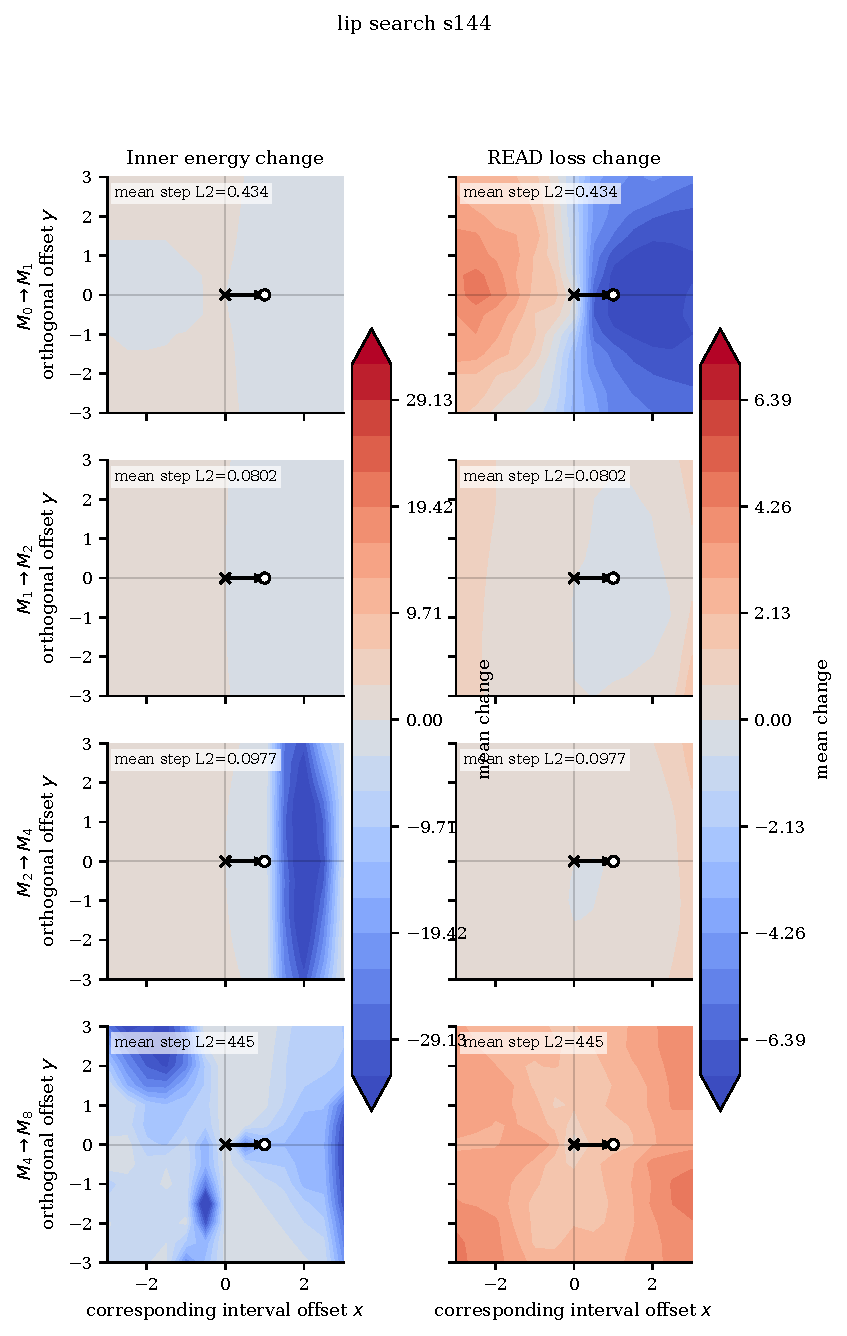
\includegraphics[width=0.82\linewidth]{figures/landscape_lip-search-s144.pdf}
  \caption{Transition-specific slices for the seed-144 Lipschitz-plus-search descendant.  The first three intervals have mean L2 norms below 0.44, but $M_4\to M_8$ has mean norm 445.1 and increases READ loss despite decreasing energy.  Coordinate scales differ by row and checkpoint.  Color scales are checkpoint-specific and saturated beyond the 97th absolute percentile.}
  \label{fig:landscape-search}
\end{figure}

\section{Discussion}
\label{sec:discussion}

\paragraph{What has been established.}
The successful \egm{} run establishes that two context-only gradient steps can encode associations under both observed serialization orders into eight prefix tokens.  Whether it uses the explicit \texttt{F}/\texttt{B} marker requires marker deletion or swap tests.  Both available reconstruction seeds exhibit a contrasting failure mode dominated by the autoregressively favored direction.  These observations support the hypothesis that the full learned-energy configuration can overcome a mismatch unresolved by the evaluated reconstruction configurations, but they do not isolate the energy objective from initialization and auxiliary losses.

\paragraph{What has not been established.}
Energy is not yet a more reliable objective.  Its three-seed mean EM is below the reconstruction baseline, and its variance is dramatically larger.  Stabilized high-accuracy runs inherit the unique successful initialization.  No current experiment isolates Lipschitz regularization, noise, or memory search as improving from-scratch convergence under matched seeds and compute.  Single-run peak accuracy should therefore not be reported as a general advantage of \egm{}.

\paragraph{Why the current Lipschitz penalty may miss the failure.}
The new frozen analysis refines this diagnosis.  The selected seed-144 Lipschitz descendant is associated with lower observed pointwise gradients at all visited states, a smaller first displacement, monotone mean energy descent, and stable $K=8$ performance.  No matched continuation isolates the penalty from continued training and checkpoint selection.  The penalty directly constrains only detached $M_K$; at the currently retained checkpoint, the observed $M_0$ gradient remains 780, far above threshold 5, while $M_2$ reaches 3.66.  The unconstrained initialization is consistent with, but does not solely explain, the still-large first step.  Endpoint gradient regularization also does not control curvature or finite-step descent by itself.  These are 12-example means at selected checkpoints, not proof of a global bound.  Applying the same strong penalty from scratch may still compete with formation of a useful update field, consistent with the failed scratch runs.

\section{Recommended Experiments}
\label{sec:recommendations}

We recommend a staged program that tests hypotheses rather than adding more coupled penalties.

\paragraph{1. Diagnose the phase transition before changing the model.}
Save or evaluate checkpoints densely around the point where seed 144 leaves the low regime.  For seeds 143--145, track orientation-conditioned EM, $E(M_k)$, $\lVert\nabla E(M_k)\rVert$, update norm, cosine similarity between energy and READ gradients, and key/value token energies at every $k$.  This can distinguish symmetry breaking, scale explosion, and a genuine representational transition.

\paragraph{2. Control the finite update, not only the local gradient.}
The immediate low-cost ablation is inner gradient clipping or normalized updates with a small grid chosen from measured displacement quantiles.  More principled alternatives are a learned positive step size with an upper bound, backtracking line search enforcing $E(M_{k+1})\leq E(M_k)$, or a trust-region penalty on $\lVert M_{k+1}-M_k\rVert$.  Run these from scratch over at least five matched seeds.  A useful primary endpoint is convergence probability to 90\% and 99\% EM, with median steps-to-threshold and failure rate, not only best EM.

\paragraph{3. Train trajectory geometry where inference visits it.}
Apply trajectory descent or Lipschitz/curvature constraints at $M_0$, $M_1$, and $M_2$, including segment samples, rather than only at $M_K$.  Normalize the constraint relative to the intended update radius so it is scale-aware.  An explicit finite-difference loss,
\begin{equation}
  \sum_k \left[ E(M_{k+1})-E(M_k)+\gamma\lVert M_{k+1}-M_k\rVert_2^2 \right]_+,
\end{equation}
directly targets the observed overshoot.  Anchor or center energy values to avoid softplus saturation and uncontrolled scale, but report whether anchoring changes the effective gradient scale.

\paragraph{4. Supervise directional utility without making WRITE query-dependent.}
Use the known synthetic structure only as an outer-loop diagnostic or auxiliary training signal.  Candidate objectives include orientation-conditioned key/value energy balance, contrastive matching between a context and its written memory, and consistency between memories written from semantically equivalent forward/backward renderings.  A particularly clean test pairs the same key--value set in both orientations and penalizes distance between the resulting final memories, while WRITE itself still sees only one context.  This asks for representation invariance without using the query or answer in the inner objective.

\paragraph{5. Use curriculum to separate acquisition from stability.}
Train first on pure forward and pure inverse batches, then increase the probability of mixed-orientation batches, or initialize from a balanced mixture of independently successful forward and inverse checkpoints.  Compare this against scratch training at matched total updates.  If curriculum reliably crosses the phase transition, the obstacle is optimization; if not, interference between directional update fields is likely central.

\paragraph{6. Treat memory search as an oracle diagnostic.}
Measure the oracle gap: the fraction of examples with a nearby lower-READ-loss perturbation, its distance, and whether the energy gradient points toward it.  Then distill those target-guided teachers into a context-only energy model and evaluate ordinary WRITE separately.  Keep configurations with teacher-for-next-step disabled distinct from those with straight-through target-guided trajectories, since the latter create a stronger train/inference mismatch.

\paragraph{7. Establish matched statistical evidence.}
For each shortlisted intervention, use at least five seeds, identical initialization policy, batch size, precision, outer schedule, $K$, inner learning rate, and checkpoint selector.  Report forward/backward EM separately, overall EM, mean and variance, success probability, and wall-clock or update budget.  Do not compare a plateau-initialized stabilized run against a scratch baseline as evidence of convergence improvement.

\section{Limitations}
\label{sec:limitations}

This report analyzes existing runs rather than a preregistered sweep.  Run counts differ across configurations, some trajectories terminated before one million steps, and checkpoints were selected by validation token accuracy.  The principal energy conclusion rests on one successful seed.  The 256-example key/value analysis is deterministic but not a full-validation confidence interval.  Additive energy offsets do not affect WRITE gradients, but multiplicative scale does; checkpoint magnitudes must be interpreted jointly with gradient norms, inner learning rate, and update norms.  Some interventions combine optimizer changes, initialization, and regularization, preventing causal attribution.  Finally, \dataset{} is synthetic and exposes orientation explicitly; transfer to natural language or longer contexts remains untested here.

\section{Conclusion}
\label{sec:conclusion}

\dataset{} exposes a specific directional weakness of autoregressive reconstruction WRITE.  Both available ordinary \gm{} seeds favor forward retrieval and substantially lower value-token reconstruction loss, yet largely fail backward retrieval.  One \egm{} configuration run handles both serialization orders and reaches 96.4\% EM.  Because initialization and auxiliary losses differ across method families, this does not isolate energy as the cause.  The solution is rare and high-gradient, semantic energy components are non-monotone, and current Lipschitz or noise interventions do not rescue convergence from scratch.  The next priority is therefore not higher peak accuracy, but controlling finite-step dynamics and measuring convergence probability across seeds while preserving query-independent inference.

\bibliographystyle{plain}
\begin{thebibliography}{1}

\bibitem{kuratov2026gradmem}
Yuri Kuratov, Matvey Kairov, Aydar Bulatov, Ivan Rodkin, and Mikhail Burtsev.
\newblock GradMem: Learning to write context into memory with test-time gradient descent.
\newblock \emph{arXiv preprint arXiv:2603.13875}, 2026.

\end{thebibliography}

\appendix
\section{Run and Reproduction Details}
\label{app:runs}

The principal successful checkpoint is
\begin{quote}\small
\path{runs/mix-N8-K2V2-V62_1M/energygradmem_llama_L4H4D256_mem8_K2_ilr0.4_energy_grad_second_stepalign0.1_iread0.1_bs_64_lr_1e-04_fp32/run_2/checkpoint-833500}.
\end{quote}
It uses seed 144, $K=2$, inner SGD learning rate 0.4, full second-order differentiation, no inner clipping, step-alignment weight 0.1, intermediate-READ weight 0.1, batch size 64, outer learning rate $10^{-4}$, eager attention, and fp32.  The best checkpoint is selected by validation token accuracy.  The key/value analysis can be reproduced with \texttt{analyze\_mix\_write\_components.py}; the report's diagnostic CSV and JSON are stored alongside this source.

\begin{table}[h]
  \caption{Principal run identifiers and selected checkpoints.  All paths are relative to the repository root and share the prefix \texttt{runs/mix-N8-K2V2-V62\_1M/}.}
  \label{tab:run-paths}
  \centering
  \scriptsize
  \begin{tabular}{lp{0.68\linewidth}l}
    \toprule
    Alias & Run suffix & Checkpoint \\
    \midrule
    \gm{} seed 143 & \path{gradmem_llama_L4H4D256_mem8_K2_ilr0.4_grad_second_bs_64_lr_1e-04_fp32_init_llama/run_1} & 69000 \\
    \gm{} seed 144 & \path{gradmem_llama_L4H4D256_mem8_K2_ilr0.4_grad_second_bs_64_lr_1e-04_fp32_init_llama/run_2} & 70000 \\
    \egm{} failed & \path{energygradmem_llama_L4H4D256_mem8_K2_ilr0.4_energy_grad_second_stepalign0.1_iread0.1_bs_64_lr_1e-04_fp32/run_1} & 308500 \\
    \egm{} successful & \path{energygradmem_llama_L4H4D256_mem8_K2_ilr0.4_energy_grad_second_stepalign0.1_iread0.1_bs_64_lr_1e-04_fp32/run_2} & 833500 \\
    \bottomrule
  \end{tabular}
\end{table}

\end{document}
